\documentclass[11pt,a4paper]{article}
\usepackage[T1]{fontenc}
\usepackage[utf8]{inputenc}
\usepackage{helvet}
\renewcommand{\familydefault}{\sfdefault}
\usepackage[margin=0.68in,top=0.55in,bottom=0.6in]{geometry}
\usepackage{microtype}
\usepackage{xcolor}
\usepackage{colortbl}
\usepackage{booktabs}
\usepackage{tabularx}
\usepackage{array}
\usepackage{enumitem}
\usepackage{titlesec}
\usepackage{fancyhdr}
\usepackage{tikz}
\usetikzlibrary{arrows.meta,positioning}
\usepackage[hidelinks]{hyperref}
\urlstyle{same}

\definecolor{ink}{HTML}{0B1220}
\definecolor{accent}{HTML}{D9542B}
\definecolor{teal}{HTML}{0F766E}
\definecolor{muted}{HTML}{64748B}
\definecolor{paper}{HTML}{F7F5F0}
\definecolor{green}{HTML}{15803D}
\definecolor{amber}{HTML}{B45309}

\titleformat{\section}{\normalsize\bfseries\color{ink}}{\thesection.}{0.45em}{}
\titlespacing*{\section}{0pt}{6pt}{2pt}
\setlength{\parindent}{0pt}
\setlength{\parskip}{3pt}
\setlist[itemize]{leftmargin=1.05em,itemsep=1pt,topsep=2pt,parsep=0pt}
\setlist[enumerate]{leftmargin=1.25em,itemsep=1pt,topsep=2pt,parsep=0pt}
\pagestyle{fancy}
\fancyhf{}
\renewcommand{\headrulewidth}{0pt}
\fancyfoot[L]{\footnotesize\color{muted}BTP Progress Report \textbullet{} Siddharth Suryavanshi \textbullet{} 2303325}
\fancyfoot[R]{\footnotesize\color{muted}\thepage/4}

\newcommand{\code}[1]{\texttt{\small #1}}
\newcommand{\done}{\textcolor{green}{\textbf{DONE}}}
\newcommand{\future}{\textcolor{amber}{\textbf{NEXT}}}
\newcommand{\good}{\textcolor{green}{\textbf{Works}}}
\newcommand{\bad}{\textcolor{accent}{\textbf{Hurts}}}

\begin{document}

\begin{center}
{\color{ink}\LARGE\bfseries Coherent by Construction}\\[2pt]
{\large A Cycle-Accurate Dual-Core MSI Cache-Coherence Simulator}\\[7pt]
{\normalsize Siddharth Suryavanshi \quad Roll 2303325 \quad Mathematics and Computing, IIT Goa}\\[2pt]
{\small BTP Progress Report \quad 22 November 2026}\\[5pt]
{\footnotesize\color{muted}Artifact: \code{model.sitar} \quad SHA-256: \code{3b9cd995\ldots463c0e} \quad Run: \code{reports/run\_20261122\_152018} \quad 18/18 PASS}
\end{center}

\vspace{-2pt}
\section{Problem Statement}
A dual-core processor with private L1 caches is only correct if every core observes a
consistent view of shared memory. The project builds a cycle-accurate Sitar model of
that problem: two cores, private split instruction/data caches, one shared instruction
memory (\code{IM}), one shared data memory (\code{DM}), two data-cache write-back
engines, and one serialized coherence bus. The data caches implement MSI snooping over
the coherence domain \code{\{dcache0, dcache1, DM\}}. The instruction caches are
read-only, so they have no write-back engine, but they are still peer-snooped over
\code{IM} to keep the two instruction-cache copies coherent.

Simulation is the right tool here because the hard cases depend on timing, not just on
the final cache state. A transaction that is correct in isolation can still fail when a
snoop, a write-back, and a processor response overlap. A cycle-accurate model makes those
windows explicit and reproducible, which is difficult to achieve on real hardware or with
a purely functional cache model.

The central difficulty is not the cache hit path; it is the race-prone miss and
ownership path. A read miss may find a dirty peer, which must supply data and downgrade
\code{M -> S}. A write miss or shared-to-modified upgrade may race with a peer that
wins exclusive ownership first, requiring an \code{RDX} recovery. A dirty line may be
invalid in the array while its data is still parked in the one-entry write buffer, so a
snoop must inspect the buffer as well as the cache. An atomic load-store must be
indivisible across both caches and memory: both copies are invalidated, dirty copies are
ordered correctly, memory performs the RMW, and the requester receives the pre-atomic
value. Finally, a cache may be snooped while waiting \code{CACHE\_DELAY} cycles before
responding to its processor, so response state must survive the snoop.

The objective is therefore a correctness-first simulator that makes these cases
observable and testable, not just a fast cache model. The prototype must complete
1,000 instructions per core in every scenario, preserve the single-writer/multiple-reader
invariant, return correct atomic old values, and account for write-backs without losing
or duplicating dirty data.

\section{Why It Matters and What the Project Aims To Do}
\textbf{Significance.} Coherence bugs are silent: a stale read or lost write can produce
wrong results long after the offending transaction. Atomics make the problem sharper
because they combine ownership, dirty-data ordering, and memory update in one operation.
Write-back buffers add a second place where dirty data can hide. These are exactly the
cases that are hard to reason about informally and valuable to reproduce in simulation.
The work is also relevant to performance: coherence traffic, bus serialization, and
memory latency can dominate runtime even when cache hit rates look healthy.

\textbf{Use and direction.} The simulator is a small architecture testbed for comparing
snooping MSI with alternatives such as directory coherence or MESI/MOESI, for studying
write-back versus write-through and blocking versus non-blocking buffers, and for
teaching why coherence protocols need explicit invariants. The direction is deliberately
conservative: establish correctness and observability first, then use the instrumented
model to explain performance rather than optimize prematurely.

\textbf{Aim and success criteria.} The aim is a cycle-accurate dual-core MSI simulator
with split caches, a six-way round-robin bus, bus-mediated atomics, peer instruction-cache
snooping, and an automated validation harness. Success means: all 18 scenarios pass;
both cores complete 1,000 instructions; zero invariant violations; zero atomic old-value
mismatches; zero both-dirty events; and consistent write-back start/done/cancel counts.
The non-goals are MESI/MOESI, directory coherence, shared L2, self-modifying code, and a
formal proof of coherence.

\section{Plan, Approach, and Subtasks}
The approach has five workstreams: (1) fix the architecture and memory model; (2) build
the parameterized set-associative cache and MSI states; (3) add bus arbitration, snooping,
and memory serialization; (4) handle atomics, write-back-buffer snoops, and instruction-
cache peer snooping; (5) validate and measure the design with a scenario matrix and plots.
Sitar supplies the discrete-event execution model; Python scripts build, run, parse,
validate, and plot each scenario.

\begin{center}
\small
\begin{tabularx}{\textwidth}{@{}p{0.56\textwidth}p{0.14\textwidth}X@{}}
\toprule
\textbf{Subtask} & \textbf{Status} & \textbf{Evidence / next step} \\
\midrule
Dual-core split-cache architecture and memory model & \done & 2 cores, 4 caches, 1 KiB IM/DM \\
MSI snooping protocol and invariant audit & \done & 18/18 scenarios, 0 violations \\
Six-way round-robin bus and typed transactions & \done & \code{BUS\_RD/\allowbreak RDX/\allowbreak UPGR/\allowbreak WB/\allowbreak ATOMIC} \\
Coherent atomic load-store and both-dirty ordering & \done & 0 old-value mismatches \\
Write-back-buffer snoop and cancellation & \done & Error 3 cancellation path \\
Instruction-cache peer snooping, no icache WB engine & \done & Static checks pass \\
Write-through staging fix and upgrade/RDX recovery & \done & 18/18 pass, cycles unchanged \\
Automated validation, metrics, and plots & \done & 18 scenarios, 8 plots \\
MESI/MOESI, directory, shared L2, formal verification & \future & Natural follow-on work \\
\bottomrule
\end{tabularx}
\end{center}

The completed work is therefore the full prototype and its validation harness. The main
remaining work is depth rather than basic functionality: richer protocols, larger core
counts, formal or randomized interleaving checks, and trace-driven workloads.

\section{Implementation, Testing, and Results}
\textbf{What was built.} \code{model.sitar} is 3,581 lines and contains the processor,
parameterized cache, write-back engine, coherence bus, dual-core integration, and memory.
Each icache is 4 sets $\times$ 4 ways $\times$ 16 B; each dcache is 2 sets $\times$ 8 ways
$\times$ 16 B. The bus has six requesters and serializes all memory traffic. Key timing
parameters are \code{CACHE\_DELAY=4}, \code{MEMORY\_DELAY=40}, and
\code{BUS\_SNOOP\_DELAY=2}. Only \code{dcache0} and \code{dcache1} instantiate write-back
engines; all four caches have peer-snoop paths.

\begin{figure}[h]
\centering
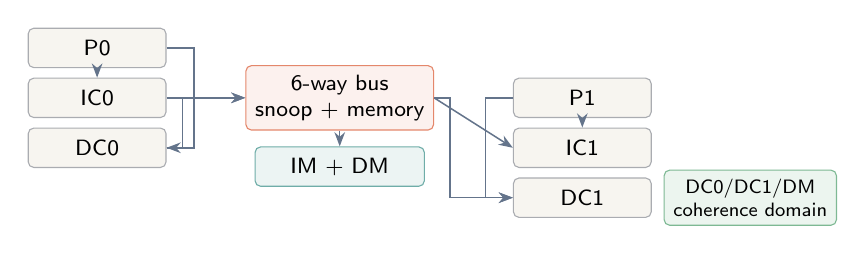
\begin{tikzpicture}[font=\footnotesize,
  comp/.style={draw=ink!35, rounded corners=2pt, fill=paper, minimum width=1.75cm, minimum height=0.5cm, align=center},
  bus/.style={draw=accent!70, rounded corners=2pt, fill=accent!8, minimum width=2.15cm, minimum height=0.75cm, align=center},
  mem/.style={draw=teal!60, rounded corners=2pt, fill=teal!8, minimum width=2.15cm, minimum height=0.5cm, align=center},
  arr/.style={-{Stealth[length=1.8mm]}, draw=muted, line width=0.55pt}]
\node[comp] (p0) {P0};
\node[comp, below=1.2mm of p0] (ic0) {IC0};
\node[comp, below=1.2mm of ic0] (dc0) {DC0};
\node[bus, right=1.0cm of ic0] (bus) {6-way bus\\snoop + memory};
\node[comp, right=1.0cm of bus] (p1) {P1};
\node[comp, below=1.2mm of p1] (ic1) {IC1};
\node[comp, below=1.2mm of ic1] (dc1) {DC1};
\node[mem, below=2.0mm of bus] (mem) {IM + DM};
\draw[arr] (p0) -- (ic0);
\draw[arr] (p0.east) -- ++(0.35,0) |- (dc0.east);
\draw[arr] (ic0.east) -- (bus.west);
\draw[arr] (dc0.east) -- ++(0.2,0) |- (bus.west);
\draw[arr] (bus.east) -- (ic1.west);
\draw[arr] (bus.east) -- ++(0.2,0) |- (dc1.west);
\draw[arr] (p1) -- (ic1);
\draw[arr] (p1.west) -- ++(-0.35,0) |- (dc1.west);
\draw[arr] (bus) -- (mem);
\node[draw=green!55, rounded corners=2pt, fill=green!8, font=\scriptsize, align=center, right=0.15cm of dc1] {DC0/DC1/DM\\coherence domain};
\end{tikzpicture}
\caption{Dual-core MSI organization. Both instruction caches snoop their peer over
\code{IM}; only the data caches have write-back engines and participate in MSI over
\code{DM}. The bus serializes all six requesters.}
\end{figure}

\textbf{Testing.} The Python harness defines 18 scenarios covering balanced, read-heavy,
write-heavy, atomic-heavy, read-only, no-data, blocking, ping-pong, locality, memory-
latency, replacement, and global-RNG cases. It builds the simulator, runs each scenario,
parses logs, checks completion and correctness, and emits CSV, JSON, summaries, and eight
plots. Deterministic per-core RNG makes address traces reproducible and independent of
bus arbitration for 17 of 18 scenarios.

\begin{center}
\small
\begin{tabularx}{\textwidth}{@{}p{0.30\textwidth}p{0.15\textwidth}p{0.15\textwidth}X@{}}
\toprule
\textbf{Scenario} & \textbf{Cycles} & \textbf{IPC} & \textbf{Key observation} \\
\midrule
Balanced & 42,733 & 0.0468 & 923 bus transactions, 232 atomics, 88.35\% IC hit \\
Atomic-heavy & 98,637 & 0.0203 & 1,265 atomics; dcache hit rate falls to 9.67\% \\
Atomic-extreme & 99,342 & 0.0201 & 2,000 atomics; near 100k-cycle limit \\
Fast vs slow memory & 14,356 / 79,235 & 0.139 / 0.025 & 5.52$\times$ runtime ratio \\
High vs low locality & 29,797 / 95,655 & 0.067 / 0.021 & Locality dominates capacity \\
\bottomrule
\end{tabularx}
\end{center}

\textbf{Validation.} The final run reports 18/18 pass, 0 failures, 0 warnings, 0 simulator
errors, 0 invariant violations, 0 atomic old-value mismatches, 0 both-dirty events, and
1,000 completed instructions per core in every scenario. Static checks confirm no icache
write-back engine and peer-snoop paths for all four caches. Write-back accounting matches
starts, completions, and cancellations.

\textbf{Good, bad, and insights.} \good: correctness, observability, deterministic
replay, and a simple protocol that is easy to audit. \bad: low aggregate IPC, a serialized
bus, synthetic workloads, a one-entry write buffer, and no formal proof. The results show
that memory latency and bus serialization dominate: fast memory completes in 14,356 cycles
versus 79,235 for slow memory, and high locality completes in 29,797 cycles versus 95,655
for low locality. Atomics are expensive because every atomic is serialized and invalidates
both data caches. Blocking versus non-blocking barely changes aggregate throughput, though
it reduces maximum write-back wait; the bus remains the bottleneck.

\textbf{Design trade-offs.} The serialized bus keeps snooping simple and gives one clear
ordering point, but it limits throughput and makes bus wait the dominant cost. Snooping
MSI is a good fit for two cores; a directory would scale better but adds complexity that
this project does not need. Write-back with write allocate reduces memory traffic, while
the write-through path is retained as a configurable alternative with explicit staging.
A blocking write buffer reduces maximum write-back wait, but it does not improve aggregate
throughput because the bus, not the buffer, is the bottleneck. These trade-offs are
intentional: the prototype favors correctness, visibility, and reproducibility over raw
performance.

\section{Limitations and Future Work}
\textbf{Limitations.} The validation is dynamic and scenario-based, not a formal proof. It
does not exhaustively enumerate every interleaving, address stream, or cache state.
Deterministic mode improves reproducibility but narrows timing diversity relative to the
global-RNG mode. The workload is synthetic, the bus is serialized, the write buffer is
one entry deep, and power/area are not modeled. These choices keep the design auditable,
but they also limit how far the performance numbers can be generalized.

\textbf{Future work.} The natural next steps are MESI/MOESI, directory coherence, a shared
L2, larger core counts, formal or randomized interleaving checks, and trace-driven
workloads. A second direction is to use the existing counters to study adaptive
replacement, write-buffer depth, and alternative arbitration policies. The current model
is a sound base for those experiments because its invariants and failure modes are
already explicit and testable.

\section{References and Use of AI}
\textbf{AI use.} AI assistance was used as a design and debugging aid, not as an
authority. The assistant helped compare architecture alternatives, reason about
\code{BUS\_ATOMIC} and write-back-buffer snooping, propose bug fixes, interpret logs, and
draft documentation. Every change was reviewed, built, and run through the full suite.
Performance and correctness numbers are taken from the generated run, not from AI
estimates; no results or logs were fabricated.

\begin{center}
\small
\begin{tabularx}{\textwidth}{@{}p{0.21\textwidth}X@{}}
\toprule
\textbf{AI model / tool} & \code{opencode CLI}; session model \code{deepseek-v4.1-flash-free} \\
\textbf{Used for} & Architecture reasoning; \code{BUS\_ATOMIC}/WB-snoop design; debugging; bug fixing; report and slide drafting \\
\textbf{Verification} & Reviewed source; rebuilt; 18/18 suite pass; zero invariant and atomic errors \\
\bottomrule
\end{tabularx}
\end{center}

\begin{sloppypar}
\textbf{References.} Gate Smashers, \emph{Computer Organization and Architecture}
(playlist), \url{https://www.youtube.com/playlist?list=PLxCzCOWd7aiHMonh3G6QNKq53C6oNXGrX};
\emph{L-3.5 What is Cache Mapping}, \url{https://www.youtube.com/watch?v=m1dA7D6c3C0};
\emph{L-3.6 Direct Mapping}, \url{https://www.youtube.com/watch?v=eObN3u3eAnU};
\emph{L-3.8 Fully Associative Mapping}, \url{https://www.youtube.com/watch?v=sLCJJdz0WAg};
\emph{L-3.10 Set Associative Mapping}, \url{https://www.youtube.com/watch?v=pFndaJARM4Q};
\emph{System Design playlist} (contains \emph{Lec-16 Write Through vs Write Back}),
\url{https://www.youtube.com/playlist?list=PLxCzCOWd7aiHanm1nA5_fMwbx5dCNFkDX};
COA roadmap, \url{https://www.gatesmashers.com/roadmaps/computer-organization-architecture}.
MIT 6.004, \emph{L25 Cache Coherence}, \url{https://www.youtube.com/watch?v=83jOKVb_HTM};
\emph{21.2.5 Cache Coherence}, \url{https://www.youtube.com/watch?v=ISaYWm8T8n4}.
CMU 15-418/15-618, \emph{Lecture 10: Snooping-Based Cache Coherence},
\url{https://www.youtube.com/playlist?list=PLpIxOj-HnDsO4Atvrp86c-4La9Mq3kMQZ};
slides, \url{https://www.cs.cmu.edu/~418/lectures/10_cachecoherence.pdf}.
Onur Mutlu, \emph{Cache Design}, \url{https://www.youtube.com/watch?v=BGaLNhyr-2Q};
\emph{Memory Hierarchy}, \url{https://www.youtube.com/watch?v=1zXDoDDkICQ};
\emph{Cache Coherence}, \url{https://www.youtube.com/watch?v=jcWemSeLiGo}.
D. Patterson and J. Hennessy, \emph{Computer Organization and Design}, 5th ed., 2014;
D. J. Sorin, M. D. Hill, and D. A. Wood, \emph{A Primer on Memory Consistency and Cache
Coherence}, 2nd ed., 2020. All links checked 22 November 2026.

\textbf{Artifacts.} Source: \code{model.sitar}; report: \code{BTP\_Report.md}; AI-use
disclosure: \code{BTP\_AI\_Use\_and\_References.md}; validation:
\code{reports/run\_20261122\_152018/}; GitHub:
\url{https://github.com/suryavanshisiddharth23033-pixel/ASS1}.
\end{sloppypar}

\section*{Appendix: Scenario Summary}
\begin{center}
\footnotesize
\begin{tabular}{@{}lrrrr@{}}
\toprule
\textbf{Scenario} & \textbf{Cycles} & \textbf{IPC} & \textbf{Atomics} & \textbf{Result} \\
\midrule
balanced & 42,733 & 0.0468 & 232 & PASS \\
global\_rng & 44,515 & 0.0449 & 261 & PASS \\
read\_heavy & 35,113 & 0.0570 & 134 & PASS \\
read\_only & 26,607 & 0.0752 & 0 & PASS \\
store\_heavy & 44,065 & 0.0454 & 159 & PASS \\
load\_extreme & 29,831 & 0.0670 & 0 & PASS \\
store\_extreme & 33,019 & 0.0606 & 0 & PASS \\
atomic\_heavy & 98,637 & 0.0203 & 1,265 & PASS \\
atomic\_extreme & 99,342 & 0.0201 & 2,000 & PASS \\
no\_data\_ops & 12,208 & 0.1638 & 0 & PASS \\
balanced\_blocking & 42,670 & 0.0469 & 232 & PASS \\
pingpong\_t3a & 47,720 & 0.0419 & 368 & PASS \\
pingpong\_blocking & 47,599 & 0.0420 & 368 & PASS \\
high\_locality & 29,797 & 0.0671 & 224 & PASS \\
low\_locality & 95,655 & 0.0209 & 225 & PASS \\
fast\_memory & 14,356 & 0.1393 & 232 & PASS \\
slow\_memory & 79,235 & 0.0252 & 232 & PASS \\
random\_repl & 43,425 & 0.0461 & 232 & PASS \\
\bottomrule
\end{tabular}
\end{center}

\textbf{Reproduction.} From the repository root, run
\code{python3 test/run\_tests.py --build}. The run writes \code{reports/run\_YYYYmmdd\_HHMMSS/}
with raw logs, CSV, JSON, summary, config, and plots. Confirm the model hash, 18 PASS
rows, zero invariant/atomic/both-dirty errors, and 1,000 instructions per core.

\vspace{2pt}
\textbf{Glossary.} MSI: Invalid, Shared, Modified. Snooping: caches observe bus
transactions and react. Dirty intervention: a modified cache supplies data to another
requester. Downgrade: modified becomes shared after supplying data. Write-back: dirty data
reaches memory on eviction or intervention. Write allocate: a store miss allocates the
block. \code{BUS\_RD}: read and share. \code{BUS\_RDX}: read exclusive. \code{BUS\_UPGR}:
upgrade shared to modified. \code{BUS\_WB}: write back a dirty block. \code{BUS\_ATOMIC}:
coherent atomic read-modify-write. IPC: instructions per cycle.

\end{document}
